\documentclass{article}

\usepackage{graphicx}
\usepackage{tikz}
\usepackage{tikzsymbols}
\usetikzlibrary{calc,patterns,shapes.geometric}
\pagestyle{empty}
\usepackage[margin=0pt]{geometry}
\geometry{papersize={14in,12in}}

\def\centerarc[#1](#2)(#3:#4:#5){\draw[#1] ($(#2)+({#5*cos(#3)},{#5*sin(#3)})$) arc (#3:#4:#5);}

\begin{document}
	\begin{figure}
		\centering
		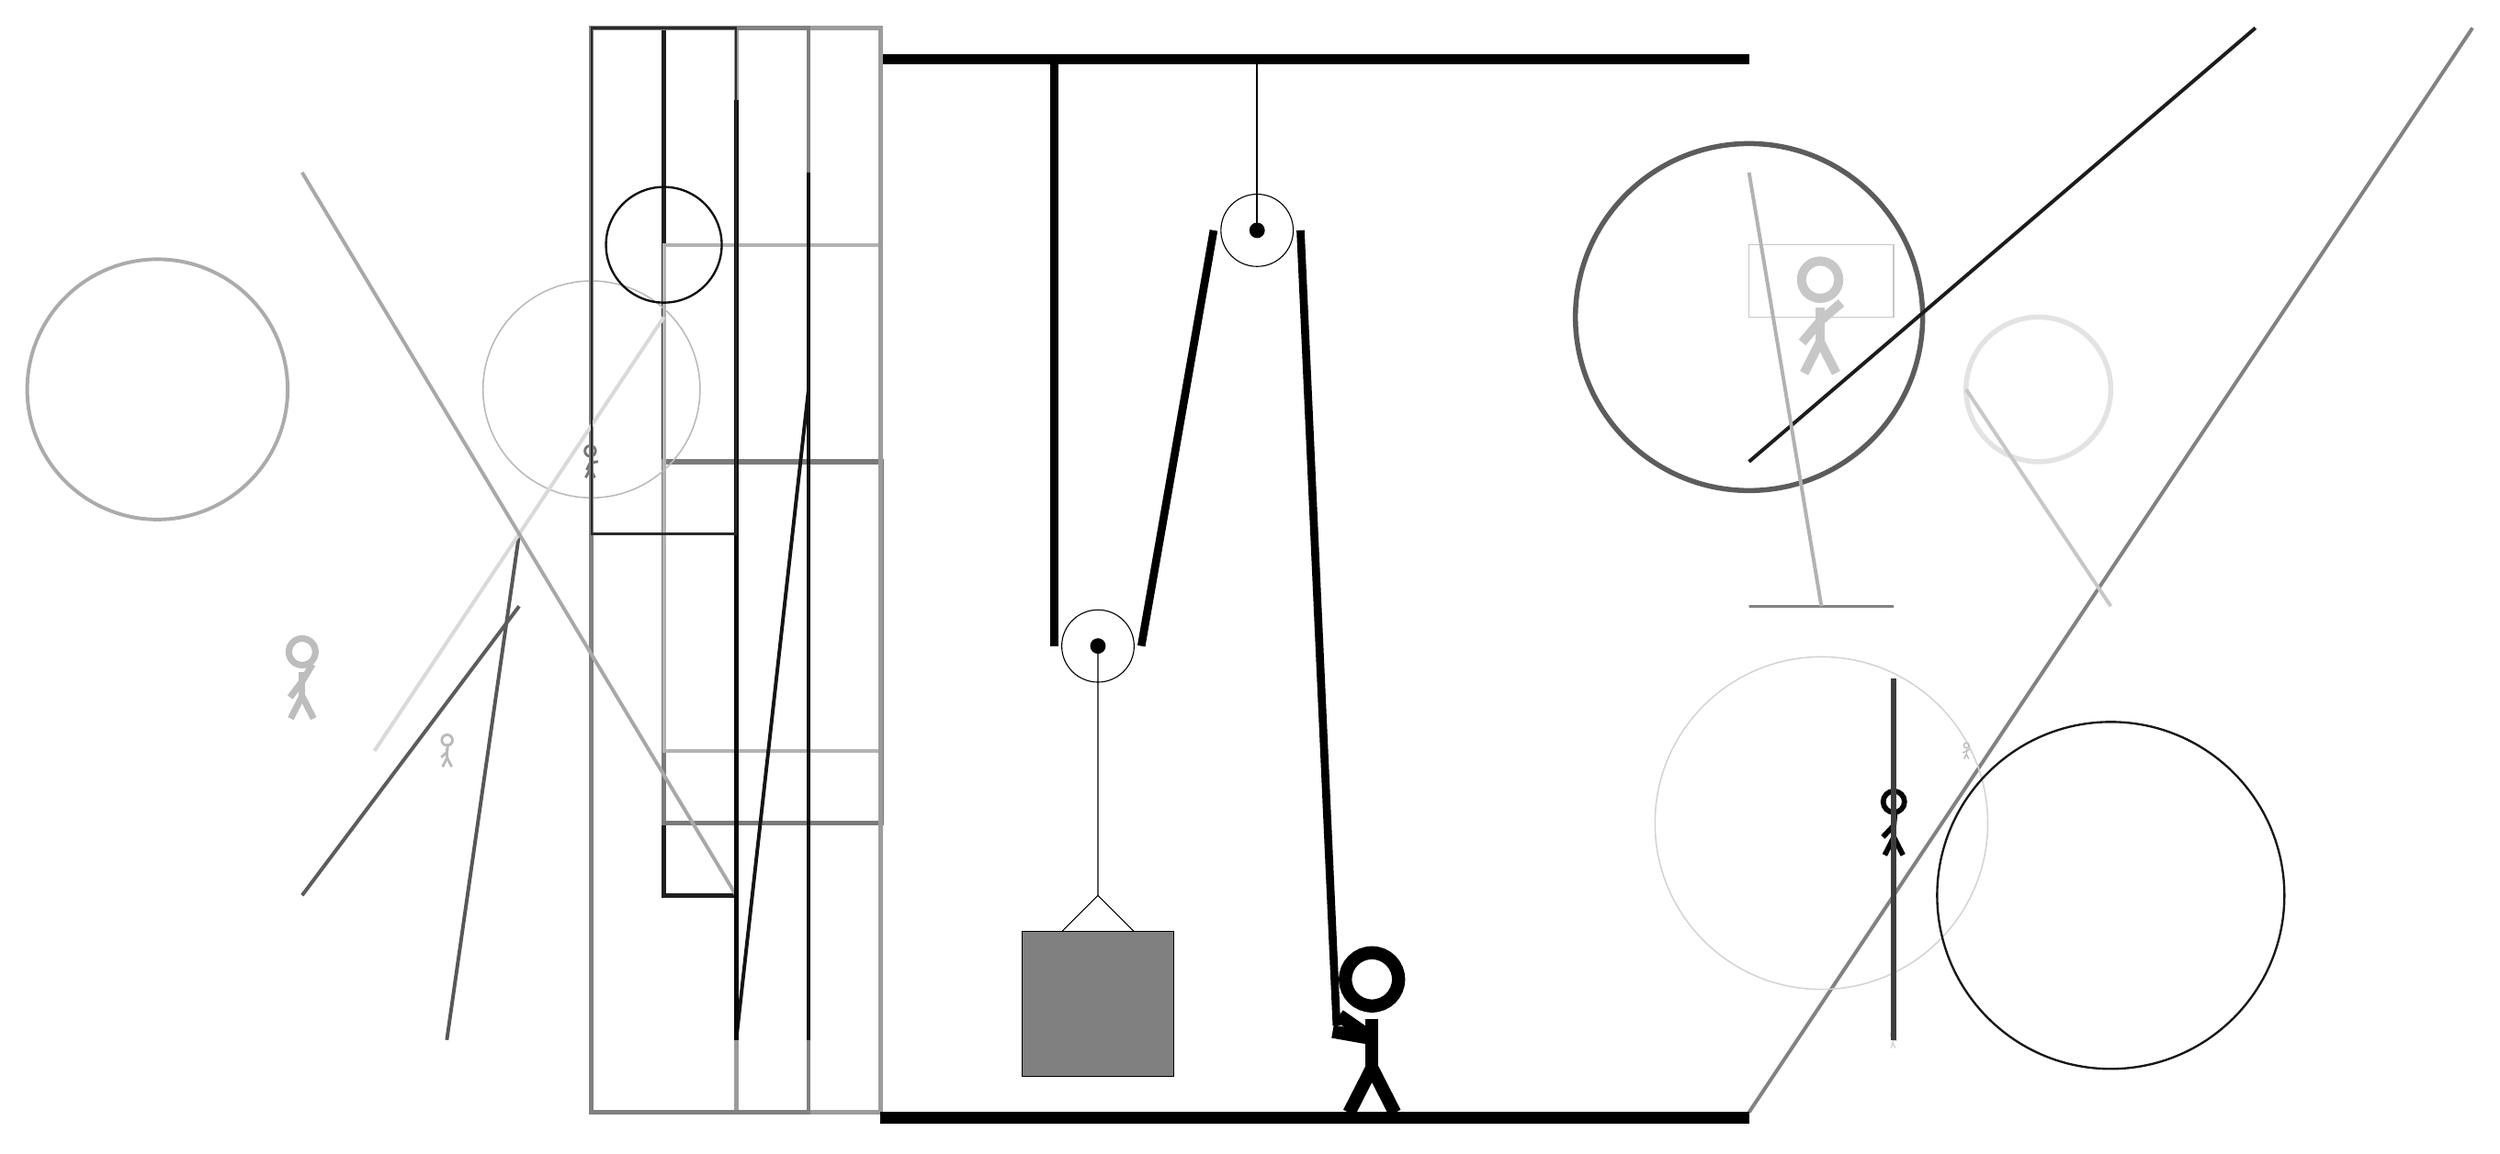
\begin{tikzpicture}
			%%%%% START %%%%%
			
			\draw[fill=black] (-2, 11.5) rectangle (10, 11.625);
			
			\draw (3.2, 9.2) circle (0.5);
			\draw[fill=black] (3.2, 9.2) circle (0.1);
			\draw[thick] (3.2, 9.2) -- (3.2, 11.5);
			
			\draw (1, 3.45) circle (0.5);
			\draw[fill=black] (1, 3.45) circle (0.1);
			
			\draw (1, 3.45) -- (1, 0.0) -- (0.5, -0.5);
			\draw (1, 0.0) -- (1.5, -0.5);
			\draw[fill=black!50] (-0.05, -0.5) rectangle (2.05, -2.5);
			
			\draw[line width=0.7mm, color=black!88] (-4, 12) rectangle (-5, 0);
			
			\draw [line width=0.7mm, color=black!11](14, 7) circle (1.0);
			\node[line width=0.7mm, color=black!26] at (-10, 3) {\Strichmaxerl[5][53][59]};
			\draw[line width=0.7mm, color=black!52] (-2, 6) rectangle (-5, 1);
			\draw[line width=0.5mm, color=black!30] (-2, 9) rectangle (-5, 2);
			\draw[line width=0.5mm, color=black!49](10, -3) -- (20, 12);
			\draw[line width=0.5mm, color=black!66](-7, 5) -- (-8, -2);
			\draw[line width=0.5mm, color=black!64](-7, 4) -- (-10, 0);
			\draw[line width=0.5mm, color=black!92](-4, -2) -- (-3, 7);
			\draw [line width=0.2mm, color=black!27](-6, 7) circle (1.5);
			\node[line width=0.4mm, color=black!54] at (-6, 6) {\Strichmaxerl[2][63][9]};
			\draw[line width=0.6mm, color=black!39] (-4, -3) rectangle (-2, 12);
			\draw[line width=0.6mm, color=black!50] (-3, 12) rectangle (-6, -3);
			\draw[line width=0.3mm, color=black!49] (12, 4) rectangle (10, 4);
			\draw[line width=0.5mm, color=black!15](-5, 8) -- (-9, 2);
			\draw [line width=0.7mm, color=black!64](10, 8) circle (2.4);
			
			\draw [line width=0.3mm, color=black!94](-5, 9) circle (0.8);
			\draw [line width=0.5mm, color=black!33](-12, 7) circle (1.8);
			\draw [line width=0.2mm, color=black!17](11, 1) circle (2.3);
			\node[line width=0.2mm, color=black!27] at (-8, 2) {\Strichmaxerl[2][42][84]};
			\draw[line width=0.5mm, color=black!89](10, 6) -- (17, 12);
			
			\node[line width=0.5mm, color=black!99] at (12, 1) {\Strichmaxerl[4][47][85]};
			
			\draw [line width=0.3mm, color=black!91](15, 0) circle (2.4);
			\draw[line width=0.5mm, color=black!34](-4, 0) -- (-10, 10);
			\draw[line width=0.7mm, color=black!97] (-4, -2) rectangle (-4, 11);
			
			\draw[line width=0.5mm, color=black!22](13, 7) -- (15, 4);
			
			\node[line width=0.2mm, color=black!16] at (12, -2) {\Strichmaxerl[1][71][6]};
			\node[line width=0.7mm, color=black!22] at (11, 8) {\Strichmaxerl[7][50][41]};
			\draw[line width=0.3mm, color=black!84] (-4, 5) rectangle (-6, 12);
			\draw[line width=0.6mm, color=black!94] (-3, 10) rectangle (-3, -2);
			\draw[line width=0.2mm, color=black!22] (12, 9) rectangle (10, 8);
			
			\node[line width=0.3mm, color=black!27] at (13, 2) {\Strichmaxerl[1][18][38]};
			\draw[line width=0.7mm, color=black!76] (12, -2) rectangle (12, 3);
			\draw[line width=0.5mm, color=black!30](10, 10) -- (11, 4);
			
			
			\draw[line width=1.1mm] (0.4, 11.5) -- (0.4, 3.45);
			\centerarc[line width=1.1mm](1, 3.45)(180:360:0.6);
			\draw[line width=1.1mm](1.6, 3.45) -- (2.6, 9.2);
			\centerarc[line width=1.1mm](3.2, 9.2)(0:180:0.6);
			\draw[line width=1.1mm](3.8, 9.2) -- (4.3, -1.8);
			
			\node at (4.7, -1.9) {\Strichmaxerl[10][-35][170]};
			
			\draw[fill=black] (-2, -3) rectangle (10, -3.15);
			
			%%%%% END %%%%%
		\end{tikzpicture}
	\end{figure}	
\end{document}